\chapter{Discussion}
\label{sec:discussion}
Etwas Text... Hier kommen noch einige Abkürzunge vor zum Beispiel \ac{ABC},\ac{WWW} und \ac{ROFL}.

\section{Erste Überschrift Tiefe 2 (section)}
blindtext

\subsection{Erste Überschrift Tiefe 3 (subsection)}
blindtext

\subsubsection{Erste Überschrift Tiefe 4 (subsubsection)}
blindtext

\section{Real-time capability}

One goal of this work is to implement a real-time capable system.
All datasets in this work are some variations of RailSem19.
This dataset consists of images of YouTube videos primarily in 25 or 30 \ac{FPS}.
The temporal dataset also includes such videos.
Therefore, the system aims to speed up to 30 \ac{FPS}.
This results in a latency of 33.33 ms or lower.
However, this is a simplified assumption based on available data rather than on a practical application.

When applied in an actual use case, the real-time capability primarily depends on the camera setup, the train velocity, the prediction, and the corresponding distances.
\autoref{fig:cameraSetup} shows a systematic camera setup with the most essential parameters, distances, and angles.
The green parts resemble the prediction with a length from the horizon line.

\autoref{func:RealTime} calculates the \ac{FPS} needed for a real-time capable system according to $d_{horizon}$ and $v_{train}$.
$d_{horizon}$ is defined by geometry of the camera setup.
Theoretically, the system is still fast enough when the train travels a distance of $d_{horizon}$ between each frame.
That corresponds to a $\lambda$ of 1.
Lamda is an additional parameter that defines how much the predicted area of the previous frame must overlap with the next frame.
Lambda must be between 0 and 1.
The lower the value, the safer the system becomes.

\begin{figure}[H]
    \centering
    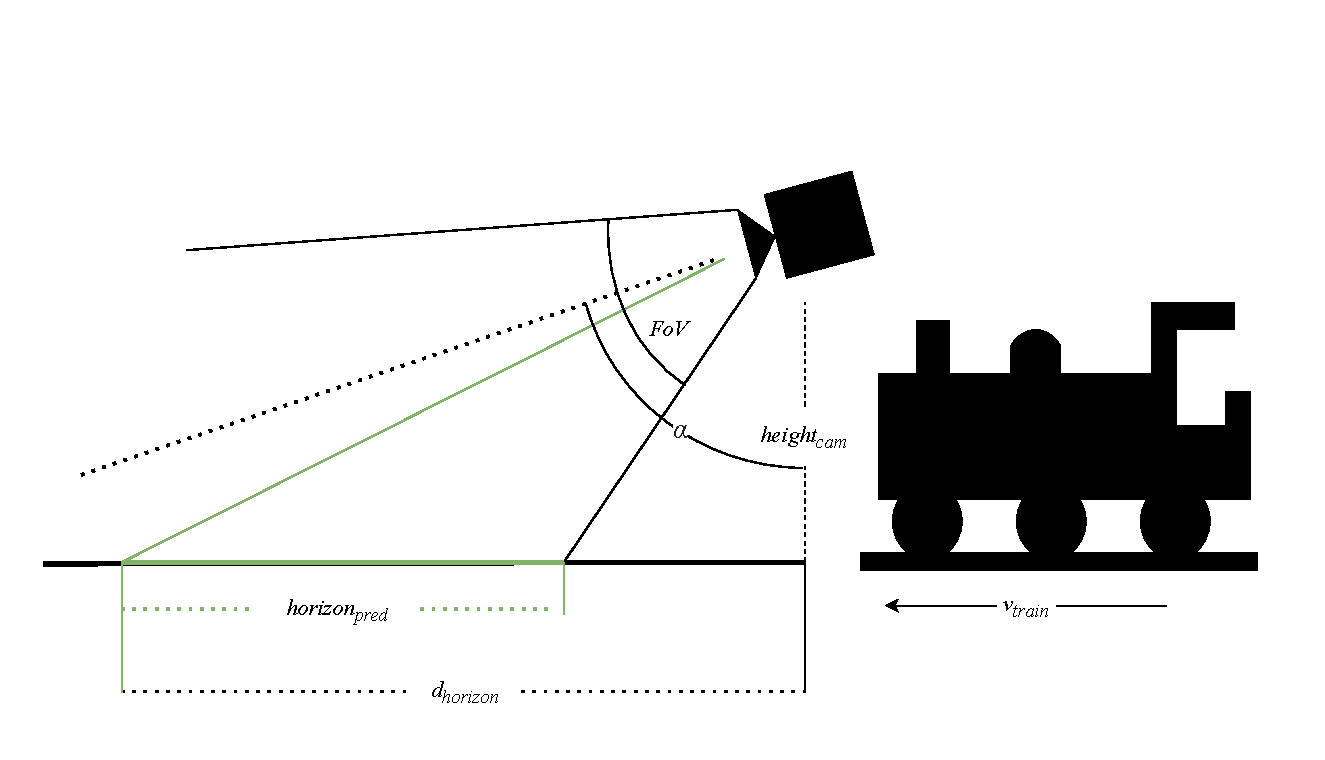
\includegraphics[width=0.8\textwidth]{PICs/discussion/Kameraaufbau.pdf}
    \caption{Camerasetup}
    \label{fig:cameraSetup}
\end{figure}

\begin{align}
    FPS = \frac{v_{train}}{d_{horizon}} \times \frac{1}{\lambda}
    \label{func:RealTime}
\end{align}

\autoref{tab:variablesForRealTime} describes realistic values when the system is prepared for trains in Austria.
A GoPro Hero 10 \cite{goproHero10} is chosen because of its integrated mounting abilities and high $FoV$.
$\alpha$ and $height_{cam}$ are assumptions for Austrian trains.
$v_{train}$ is the fastest speed a train can drive in Austria \cite{geschwindigkeitZugAustria}.
Previous predictions like in \autoref{fig:autocropVideoComparison} lead to the assumption of $horizon_{pred}$.
480 pixels are roughly a third of the image that fits most predictions in this work.
\autoref{func:FPSValues} shows that only a speed of 5.1 \ac{FPS} is needed for a practical use case with the assumed parameters.
However, to increase safety, the overlap factor $\lambda$ is set to 0.17, which results in a frame rate of 30 \ac{FPS}.
Also interesting is that with this frame rate and the highest possible train speed, the distance traveled between frames is 2.45 m, as shown in \autoref{func:distanceBetweenFrameswith30FPS}.

\begin{table}[H]
    \centering
    \begin{tabular}{|l|c|c|}
    %\begin{tabular}{| p{0.3\linewidth} | p{0.6\linewidth} |}
        \hline
        \textbf{Parameters} & \textbf{Variables} & \textbf{Assumptions}\\
        \hline
        Camera model & & GoPro Hero 10 Black \cite{goproHero10} \\
        \hline
        Vertical Field of View & $FoV$ & $93^\circ$ \cite{goproHero10} \\
        \hline
        Camera mounting angle & $\alpha$ & $90^\circ$ \\
        \hline
        Camera mounting height & $height_{cam}$ & 4 m \\
        \hline
        Train speed & $v_{train}$ & 265 km/h \cite{geschwindigkeitZugAustria} $ \Leftrightarrow\ $ 73.61 m/s\\
        \hline
        Predicted horizon line & $ horizon_{pred} $ & 480 pixel from top \\
        \hline
        Overlap factor & $\lambda$ & 0.17 \\
        \hline
    \end{tabular}
    \caption{Variables for real time calculation}
    \label{tab:variablesForRealTime}
\end{table}

\begin{align}
    d_{horizon} = \tan \left( \left( \frac{image_{height} - horizon_{pred}}{image_{height}} \times FoV \right) + \alpha - \frac{FoV}{2} \right) \times height_{cam}
    \label{func:dHorizon}
\end{align}

\begin{align}
    d_{horizon} = \tan \left( \left( \frac{720 - 480}{720} \times 93 \right) + 90 - \frac{93}{2} \right) \times 4 = 14.42 \, {m}
    \label{func:dHorizonValues}
\end{align}

\begin{align}
    FPS = \frac{v_{train}}{d_{horizon}} \times \frac{1}{\lambda} = \frac{73.61}{14.42} \times \frac{1}{1} = 5.1
    \label{func:FPSValues}
\end{align}

\begin{align}
    FPS = \frac{v_{train}}{d_{horizon}} \times \frac{1}{\lambda} = \frac{73.61}{14.42} \times \frac{1}{0.17} = 30
    \label{func:FPSValuesOverlap}
\end{align}

\begin{align}
    d_{frames} = \frac{v_{train}}{FPS} = \frac{73.61}{30} = 2.45 \, {m}
    \label{func:distanceBetweenFrameswith30FPS}
\end{align}

\vspace{1cm}

\begin{figure}[H]
    \centering
    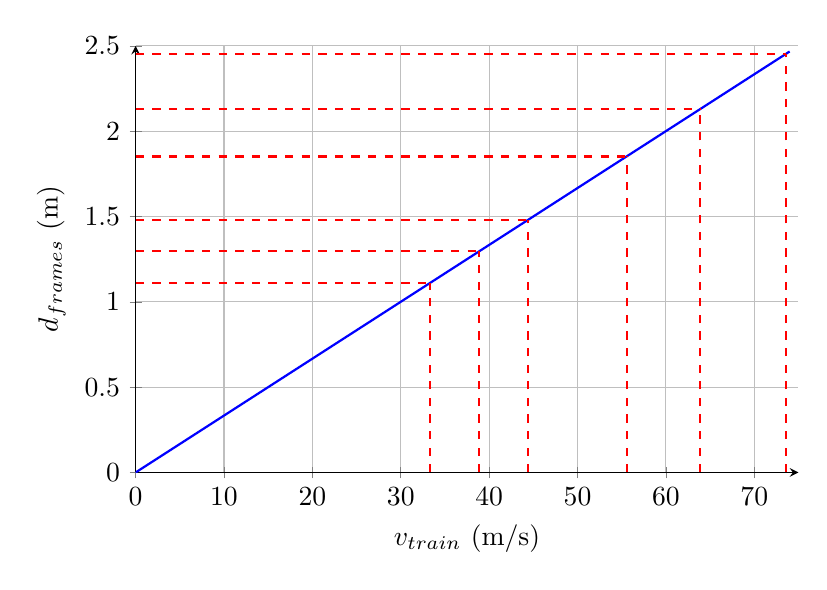
\begin{tikzpicture}
    \begin{axis}[
        width=10cm, height=7cm, % Größe des Graphen
        xlabel={$v_{train}$ (m/s)},
        ylabel={$d_{frames}$ (m)},
        xmin=0, xmax=75, % Begrenzung der x-Achse
        ymin=0, ymax=2.5, % Begrenzung der y-Achse
        grid=major,
        axis lines=left,
        legend style={at={(0.95,0.05)},anchor=south east},
        ]
        % Graph der Funktion y = 1/30 * x
        \addplot[blue, thick, domain=0:74, samples=100] {1/30 * x};
        
        % Vertikale und horizontale Linien für die gewünschten Geschwindigkeiten
        % 120 km/h = 33.33 m/s
        \draw[red, thick, dashed] (axis cs:33.33,0) -- (axis cs:33.33,1.111); % vertikal
        \draw[red, thick, dashed] (axis cs:0,1.111) -- (axis cs:33.33,1.111); % horizontal
        
        % 140 km/h = 38.89 m/s
        \draw[red, thick, dashed] (axis cs:38.89,0) -- (axis cs:38.89,1.2963); % vertikal
        \draw[red, thick, dashed] (axis cs:0,1.2963) -- (axis cs:38.89,1.2963); % horizontal
        
        % 160 km/h = 44.44 m/s
        \draw[red, thick, dashed] (axis cs:44.44,0) -- (axis cs:44.44,1.4813); % vertikal
        \draw[red, thick, dashed] (axis cs:0,1.4813) -- (axis cs:44.44,1.4813); % horizontal
        
        % 200 km/h = 55.56 m/s
        \draw[red, thick, dashed] (axis cs:55.56,0) -- (axis cs:55.56,1.8519); % vertikal
        \draw[red, thick, dashed] (axis cs:0,1.8519) -- (axis cs:55.56,1.8519); % horizontal
        
        % 230 km/h = 63.89 m/s
        \draw[red, thick, dashed] (axis cs:63.89,0) -- (axis cs:63.89,2.1297); % vertikal
        \draw[red, thick, dashed] (axis cs:0,2.1297) -- (axis cs:63.89,2.1297); % horizontal
        
        % 265 km/h = 73.61 m/s
        \draw[red, thick, dashed] (axis cs:73.61,0) -- (axis cs:73.61,2.4537); % vertikal
        \draw[red, thick, dashed] (axis cs:0,2.4537) -- (axis cs:73.61,2.4537); % horizontal
        
    \end{axis}
    \end{tikzpicture}
    \caption{Ratio between the train's speed and the distance it drives between frames with 30 \ac{FPS}. Red lines are top speeds of all different trains from Austria: 120 km/h, 140 km/h, 160 km/h, 200 km/h, 230 km/h, 265 km/h, \cite{geschwindigkeitAllTrainsAustria}}
    \label{fig:ratioSpeedDistanceBetweenFrames}
\end{figure}

\autoref{tab:temporalModelsResultsLatency} shows that the fastest temporal model is CNN\_FLAT\_FC in FP16.
Compared to the single-frame-based model, this method suffers from an increased latency, which is too high for inferring videos with 30 \ac{FPS}.
According to the calculations of \autoref{func:FPSValues}, the theoretical frame rate needed for real-time is 5.1 \ac{FPS}, which corresponds to a latency of 196.08 ms.
Since all temporal FP16 models have latencies below that, they are all theoretically real-time-capable.
FP32 models are too slow.

However, various methods could allow higher frame rates in practical operations.
An increase in speed can be achieved by utilizing a MobileNet backbone.
\autoref{tab:temporalModelsResultsLatency} shows that this increases speed significantly and is within the limits of real-time capability when inferring 30 \ac{FPS} videos.
Evaluations of these models' accuracy are out of this work's scope.

A frame rate of 5.1 \ac{FPS} is an extreme case with an overlap factor of 1, which decreases the possible safety of the system.
That leads to the thought that the optimal trade-off must be found between the overlap of the predicted areas of consecutive frames and the frame rate.
For example, only every third or fourth frame can be used, which reduces the frame rate and increases the allowed latency.

An additional advantage of only inputting every third or fourth frame into the model is that the temporal context window increases even when the length of the sliding window remains the same.
Even though information between frames is lost, ten frames would cover a window of 30 or 40 frames.
Furthermore, using this technique decreases the number of frames in which the train is located directly over the switch, resulting in a smaller time frame that needs to be bridged.